% questions.tex —— 1958 年·北京卷 · 题目内容片段（无答案）
% 由 tools/generate_projects.py 依来源总账自 1958/1958_北京_数学真题_试题.md 生成，勿手改（改源 MD 后重跑）


\gkpart{一}

\begin{question}
\gkti{1}解方程 $x-5=\sqrt{x+7}$。（5 分）

\end{question}
\begin{question}
\gkti{2}已知 $\lg 2=0.3010$，试利用对数性质判定 $2^{7}\cdot 8^{11}\cdot 5^{10}$ 是几位数。（5 分）

\end{question}
\begin{question}
\gkti{3}由 $50$ 个不同的元素中选 $47$ 个，问有多少种选法？（6 分）

\end{question}
\begin{question}
\gkti{4}求 $\tan\left(\arctan\dfrac{5}{6}-\arctan\dfrac{3}{8}\right)$ 之值。（6 分）

\end{question}
\begin{question}
\gkti{5}在 $\triangle ABC$ 中，已知 $\angle A=135^\circ$，$\angle B=15^\circ$，$C=1$。问三角形的最大边长是多少？（6 分）

\begin{gktip}
\textbf{源注}：原卷印作大写斜体「$C=1$」，按题意指 $\angle C$ 的对边 $AB$ 之长（通常记作小写 $c$）；转录保留原卷写法。
\end{gktip}

\end{question}
\begin{question}
\gkti{6}过球面上的两个不同点能作几个大圆？为什么？（6 分）

\end{question}
\begin{question}
\gkti{7}自 $30^\circ$ 的二面角的一个面上一点 $A$ 作另一个面的垂线，垂足是 $B$，若已知 $AB$ 的长是 $a$，求 $A$ 点到二面角的棱的距离。（6 分）

\end{question}
\begin{question}
\gkti{8}已知二次函数 $y=3+2x-x^{2}$。（15 分）

（1） 问 $x$ 在什么范围内 $y>0$？又 $x$ 在什么范围内 $y<0$？

（2） 求出这个函数图象的顶点坐标和对称轴方程。

（3） 画出这个函数的图象。

\end{question}
\gkpart{二}

\begin{question}
\gkti{9}设 $\sin\alpha$ 和 $\sin\beta$ 是方程

\nopagebreak[4]
\[
x^{2}-\left(\sqrt{2}\cos 20^\circ\right)x+\left(\cos^{2}20^\circ-\frac{1}{2}\right)=0
\]

的两根，其中 $\alpha$，$\beta$ 是锐角，求 $\alpha$，$\beta$ 的度数。（15 分）

\end{question}
\gkpart{三}

\begin{question}
\gkti{10}有甲、乙两容器，甲容器是直圆柱形，高 $2$ 寸，底半径 $1$ 寸，乙容器是直圆锥形（锥底向上）高 $2$ 寸，底面半径 $2\sqrt{3}$ 寸，若将甲容器灌满水，然后把甲容器的一部分水倒入乙容器使得甲乙两容器的水面一样高，问这时水面的高度是多少？（15 分）

\end{question}
\gkpart{四}

\Needspace{0.4\textheight}
\begin{question}
\gkti{11}已知 $\widehat{AB}$ 是 $\odot O$ 上含 $120^\circ$ 的弧，过 $A$，$B$ 两点所引 $\odot O$ 的切线交于 $C$，$\odot M$ 是与 $\widehat{AB}$，$AC$，$BC$ 都相切的圆，求证 $\odot M$ 的周长等于 $\odot O$ 的周长的 $\dfrac{1}{3}$。（15 分）
\nopagebreak[4]
\begin{center}% 1958 年北京卷第 11 题：⊙O、过 A、B 两点的切线及其交点、与弧 AB 和两切线相切的圆 ⊙M（按源卷布局；切线交点 C 原卷图中未标注字母，故不标）
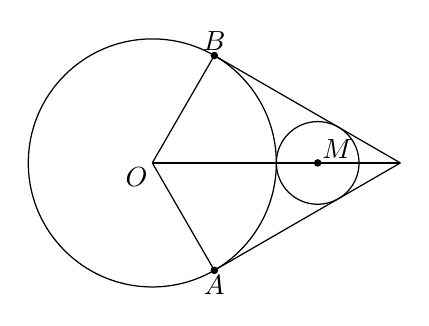
\begin{tikzpicture}[scale=1.05, line width=0.45pt,
  every node/.style={inner sep=1.5pt}]
  \coordinate (O) at (0,0);
  \coordinate (B) at (0.75,1.299);
  \coordinate (A) at (0.75,-1.299);
  \coordinate (M) at (2,0);
  \coordinate (C) at (3,0);
  \draw (O) circle (1.5);
  \draw (M) circle (0.5);
  \draw (O) -- (C);
  \draw (O) -- (B);
  \draw (O) -- (A);
  \draw (B) -- (C);
  \draw (A) -- (C);
  \fill (A) circle (1.3pt);
  \fill (B) circle (1.3pt);
  \fill (M) circle (1.3pt);
  \node[anchor=north east] at (O) {$O$};
  \node[anchor=south] at (B) {$B$};
  \node[anchor=north] at (A) {$A$};
  \node[anchor=south west] at (M) {$M$};
\end{tikzpicture}
\end{center}
\nopagebreak[4]

\end{question}